\chapter{Multiple Instance Learning}
\section{Fundamentals}
The term multiple instance learning originates from \cite{MILfirstly} and in \cite{mandlik}, authors proposed following nomenclature for MIL, which will be reviewed and gladly used in our work. \\
In standard machine learning problems each sample is represented by a fixed vector $\boldsymbol{x}$ of observations, however in multiple instance learning (MIL) it is dealt with samples which are represented by a set of vectors. These vectors are called \emph{instances} and come from an instance space $\mathcal{X}$, for example $\mathbb{R}^n$. Sets of these instances are called \emph{bags} and come from bag space $\mathcal{B} = \mathcal{P}_F\left(\mathcal{X}\right)$, where $\mathcal{P}_F\left(\mathcal{X}\right)$ denotes all finite subsets of $\mathcal{X}$. With this in mind, we can easily write down any bag as $b = \left\lbrace \boldsymbol{x} \in  \mathcal{X} \right\rbrace_{\boldsymbol{x} \in b}$. Each bag $b$ can be arbitrarily large or empty thus the size of bag is defined in the form $\vert b\vert \in \mathbb{N}_0$. There may exist intrinsic labeling of instances, but we are only interested in labeling at the bag levels. Bag labels come from a finite set $\mathcal{C}$ and what we want in MIL is learning a predictor in the form $f_{\boldsymbol{\theta}}: \mathcal{B}\left(\mathcal{X}\right) \rightarrow \mathcal{C}$ which can also be rewritten in the form $f_{\boldsymbol{\theta}}\left(\left\lbrace \boldsymbol{x}\right\rbrace_{\boldsymbol{x}\in b}\right)$. In contrast to ML, where a predictor is learned in the form  $f_{\boldsymbol{\theta}}: \mathbb{R}^n \rightarrow \mathcal{C}$.  We consider supervised setting, in which each sample of the dataset is attributed a label. We can denote available data by notation $\mathcal{D} = \Big\lbrace \left(b_i, y_i\right) \in \mathcal{B}\times\mathcal{C} \ | \ i \in \big\lbrace 1,2,\dots,\vert \mathcal{D} \vert \big\rbrace \Big\rbrace$, where $\vert \mathcal{D} \vert$ apparently denotes the size of $\mathcal{D}$. 
\begin{figure}[h]
	\centering
	\subfloat[Standard machine learning]
	{{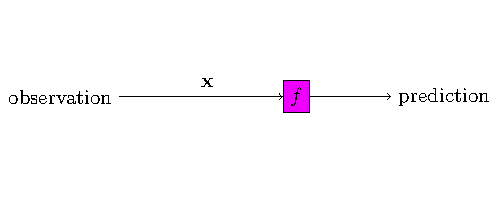
\includegraphics[width=8.0cm]{plots/Images/tikzit_image1} }}%
	\subfloat[Multiple instance learning]
	{{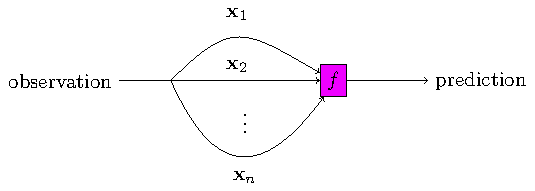
\includegraphics[width=8.0cm]{plots/Images/tikzit_image3} }}%
	\caption{The difference between standard ML and MIL \cite{mandlik}. Standard ML is special case of MIL with $\vert b \vert = 1$. }%
	\label{ggm}%
\end{figure}
\section{Embedded-space paradigm}
Embedded space paradigm \cite{mandlik} defines a vector space for bag representation and specify a mapping from each bag $b\in \mathcal{B}$ to this space. Assume that target vector space is $\R^d$, then partial mapping $\phi_i$: $\mathcal{B} \to \R,~~\forall i=1,2\dots d$~~is defined and overall embedding $\boldsymbol{\phi}: \mathcal{B} \to \R^d $ is given by
\begin{equation}
	\boldsymbol{\phi}(b) = \left(\phi_1(b), \phi_2(b), \dots, \phi_m(b)\right).
\end{equation}
Mappings $\phi_i$ are instrumentals towards extraction and suitable aggregation of information on the level of instances. They can be defined via some instance transformation $k:\mathcal{X}\to \R^d$ and aggregation function $g:\mathcal{P}_F\left(\R^d\right) \to \R^s$ in the form 
\begin{equation}
	\phi_i(b)=g\left( k\left\{\boldsymbol{x}\right\}_{\boldsymbol{x} \in b}\right).
\end{equation}
On the resulting embedded representation of bag samples can be applied any standard machine learning algorithm, which is training bag-level classifier $f_{\boldsymbol{\theta}}^B :\R^s \to \mathcal{C}$ using adjusted dataset $\mathcal{D}_{\mathrm{ES}}~=~\Big\lbrace \left(\phi(b_i), y_i\right)~\in~\R^s\times\mathcal{C}~\ ~|~\ i~\in~\big\lbrace 1,2,\dots,\vert\mathcal{D}\vert\big\rbrace\Big\rbrace$. The most used aggregation functions are minimum, maximum or mean value.
\section{Training}\label{MILtraining}
Authors of \cite{mandlik} proposed a versatile, unified framework called HMill (Hierarchical multi--instance learning library) for model definition, training and even implemented this functionality in \emph{Julia} programming language. Furthermore, the framework was published as an open--source project entitled \emph{Mill.jl} under MIT license. The aim of this work does not lie in rigorous derivation of the MIL model, since it is fairly complicated and requires considerable amount of work. Considering that, we settle with the MIL model being a neural network (NN) utilizing aggregation functions on the level of instances and we refer to \cite{mandlik} for more details about the model definition and its composition.   \\
Learning of the MIL model $f_{\boldsymbol{\theta}}$ is also supervised, a specific case called binary classification, and therefore accomplished by minimizing standard cross--entropy 
\begin{equation}\label{crossentropy52}
	\min_{\boldsymbol{\theta}}- \mathbb{E}_{p_{\mathrm{data}}(\boldsymbol{x},y) }\left[\log \frac{\exp\left({f_{\boldsymbol{\theta}}\left(\boldsymbol{x}\right)[y]}\right)}{\sum_{i=1}^C\exp\left({f_{\boldsymbol{\theta}}\left(\boldsymbol{x}\right)[y_i]}\right)} \right],
\end{equation}   
already mentioned in section \ref{discriminative_modelinmg}. This is very important for us and we will take advantage of that in our experiments.
 
\section{Cross--validation on MIL datasets}\label{experimentCV}
For testing MIL, we have available four datasets, namely Musk1, Musk2, Tiger and Fox. All of them will be used to assess performance of the MIL model.
\subsection{Setup}
In this experiment, datasets are 100 times randomly split into 2 sets in advance, train and test sets, with 80\% of observations being in train set and 20\% of observations belonging to test set. For a future simplification, let a number of random splits be denoted by $r$, thus $r=100$.  We fit the model on train set, then we evaluate the prediction error on the train data via cross--entropy \ref{crossentropy}. The objective here is to plot the prediction error dependency on the model complexity. Smaller number of random splits $r$ were tested, but obtained results were too noisy. For this reason, such high $r$ was selected, although the experiment became noticeably expensive to compute.    \\

\begin{figure}[h]
	\centering
	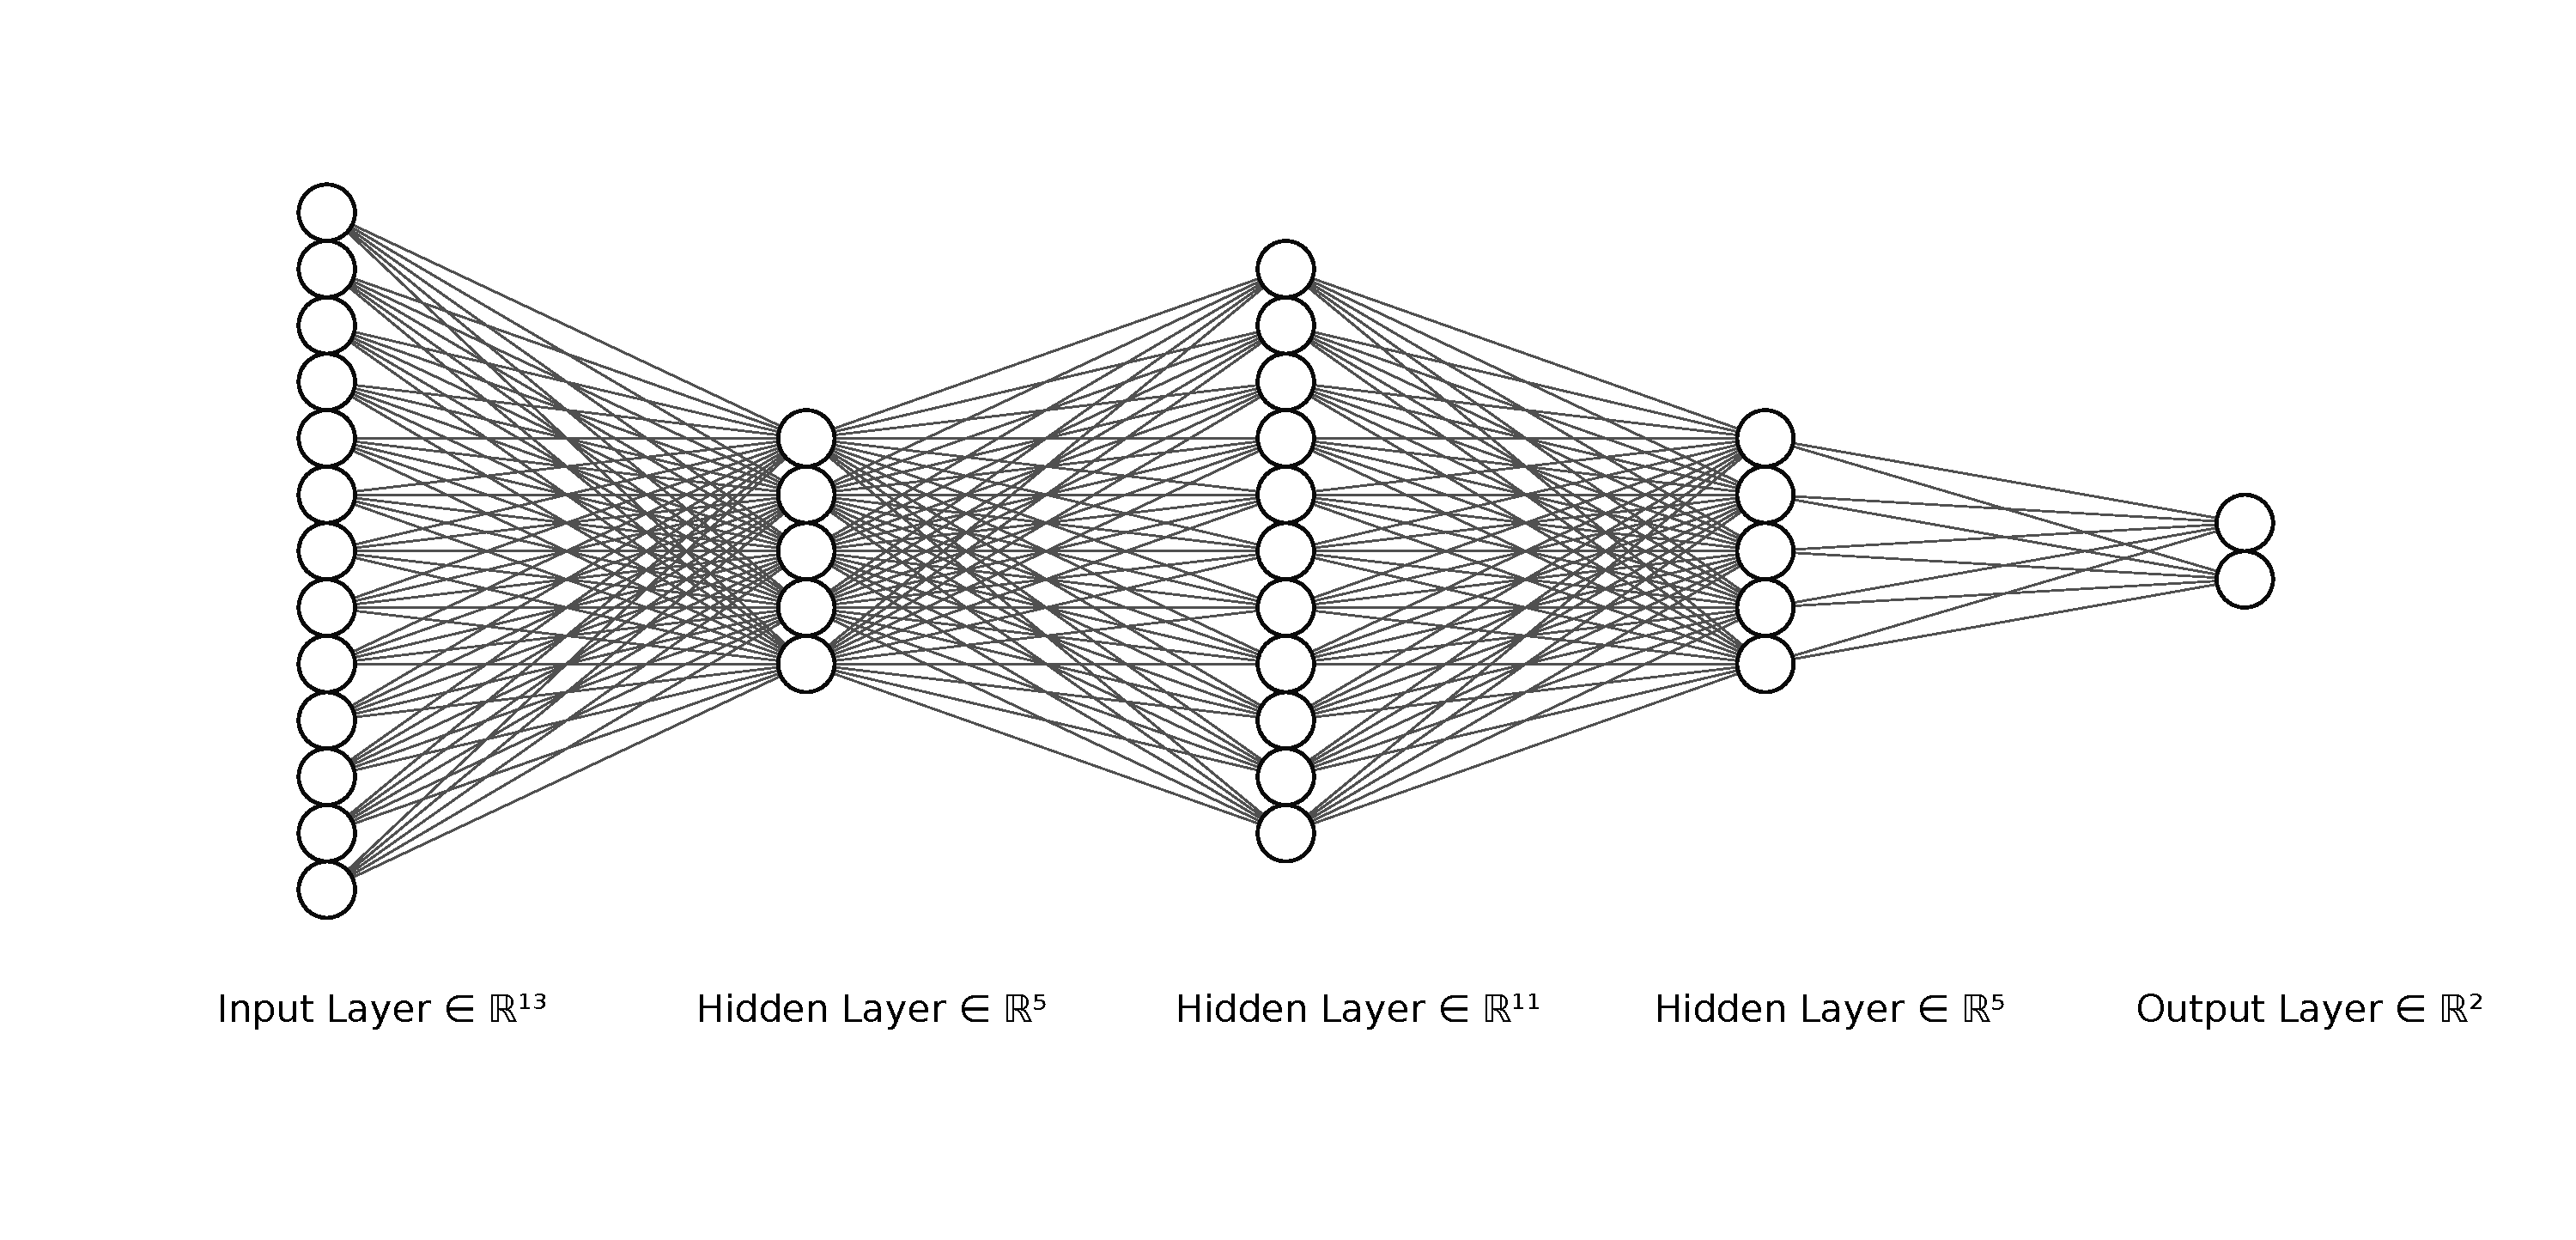
\includegraphics[width=16.0cm, trim={4cm 4.0cm 0.5cm 3.5cm},clip]{plots/Images/nn.pdf}
	\caption{NN example for $z=5$, where input and output layer are only illustrative.}
	\label{NN}
\end{figure}

\begin{para}{Model Complexity}As was mentioned in section \ref{MILtraining}, defining such model for the MIL problem is very complex task, therefore choosing a right model complexity metric is not trivial. Consider a neural network consisting of input layer, 3 hidden layers $h_1\in \R^z, h_2\in \R^{2z+1}, h_3\in \R^z$ and output layer. Then $z \in \left\{1,2,3\dots,20 \right\}$ was selected as model complexity metrics, because this is one of the easiest ways, how to control complexity of the defined MIL model. To gain a better insight, example of such NN is illustrated in Figure \ref{NN}, however this is not the exact NN used in HMill.
\end{para}     

\begin{para}{Prediction Error}
For prediction error metrics will be simply used standard cross--entropy loss  as outlined at the beginning of this section.  There is no need for any trickier objective. Let the total cross--entropy loss evaluated on $k^{\mathrm{th}}$ random split for fixed $z$ be denoted by $\pazocal{L}_k(z)$, then the estimated prediction error is given by 
\begin{equation}
	\widehat{\mathrm{Err}}(z) = \frac{1}{r}\sum_{k=1}^r \pazocal{L}_k(z).
\end{equation}
\end{para}
\vspace{1cm}

To summarize,  we fit 100 models for selected $z$ on train data and evaluate prediction error for all of them on test data, then we take mean value. This process is repeated for each $z~\in~\left\{1,2,3\dots,20 \right\}$, giving 2000 models in total. 
\subsection{Results}
As can be seen in Figure \ref{CV}, obtained results are totally expected. The prediction error evaluated on the training data for higher model complexity approaches zero. However, testing data give oscillating curves with an increasing trend (with a little exception of Musk1), therefore the model selection is necessary. This applies for each dataset.  In addition, following table \ref{tab:resultsCV} numerically summarizes the results evaluated on testing data. 

\begin{figure}[h]
	\centering
	\subfloat[CV for dataset Musk1.]
	{{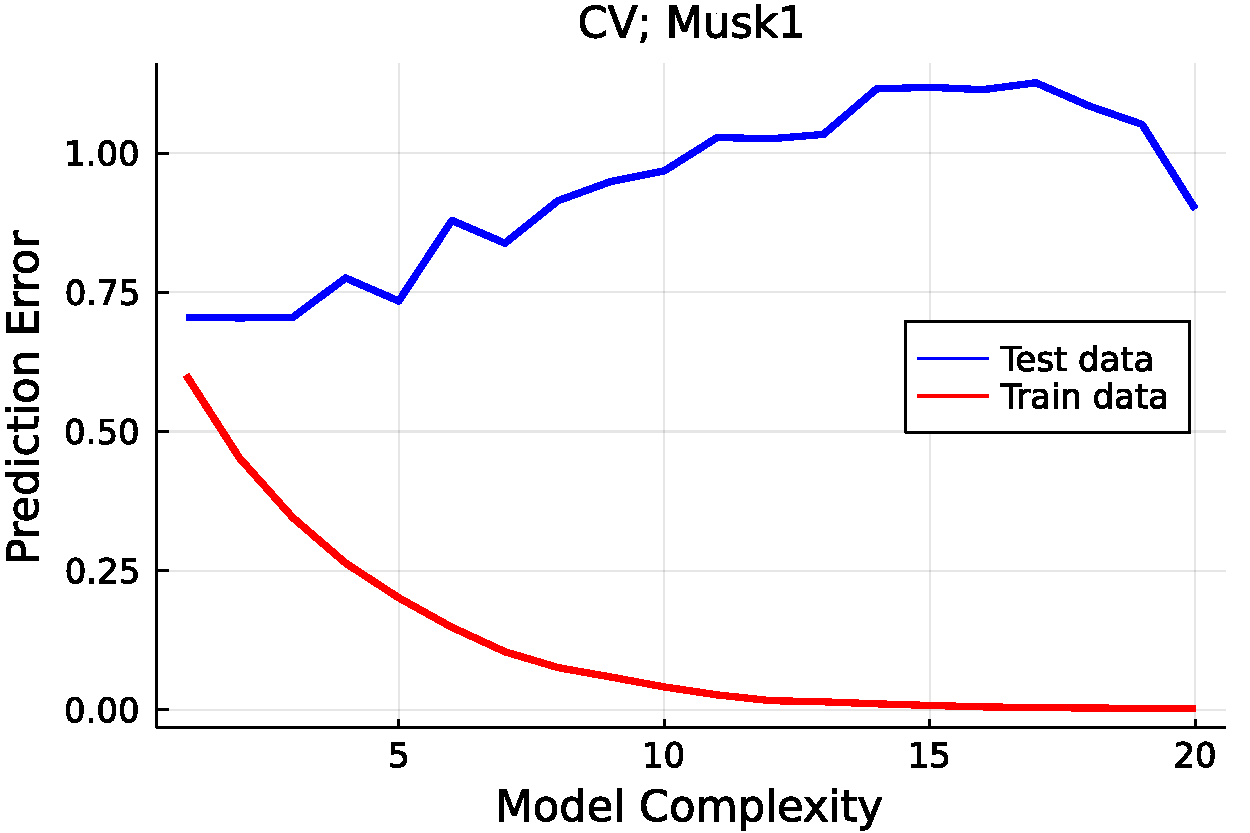
\includegraphics[width=8.0cm]{plots/Images/KFCV_Musk4.pdf} }}%
	\subfloat[CV for dataset Musk2.]
	{{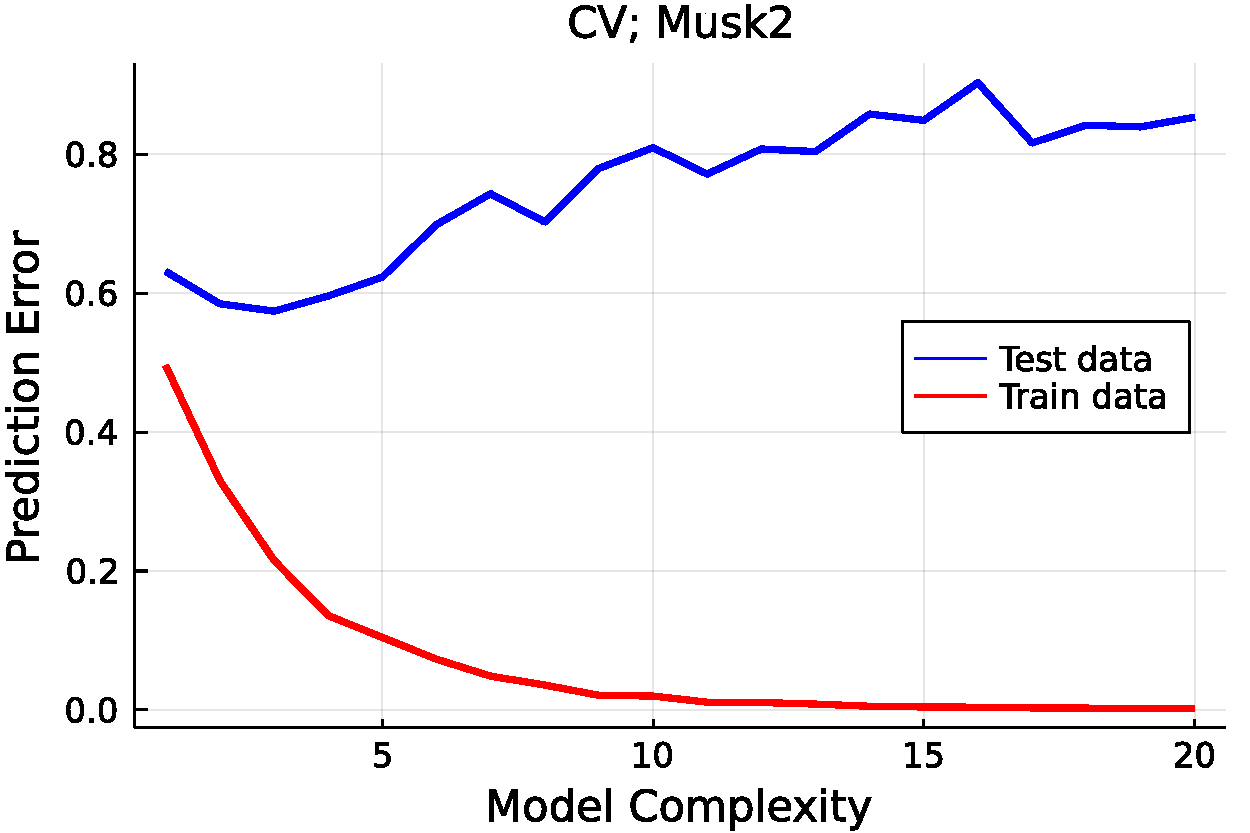
\includegraphics[width=8.0cm]{plots/Images/KFCV_Musk2.pdf} }}%
	\
	\subfloat[CV for dataset Fox.]
	{{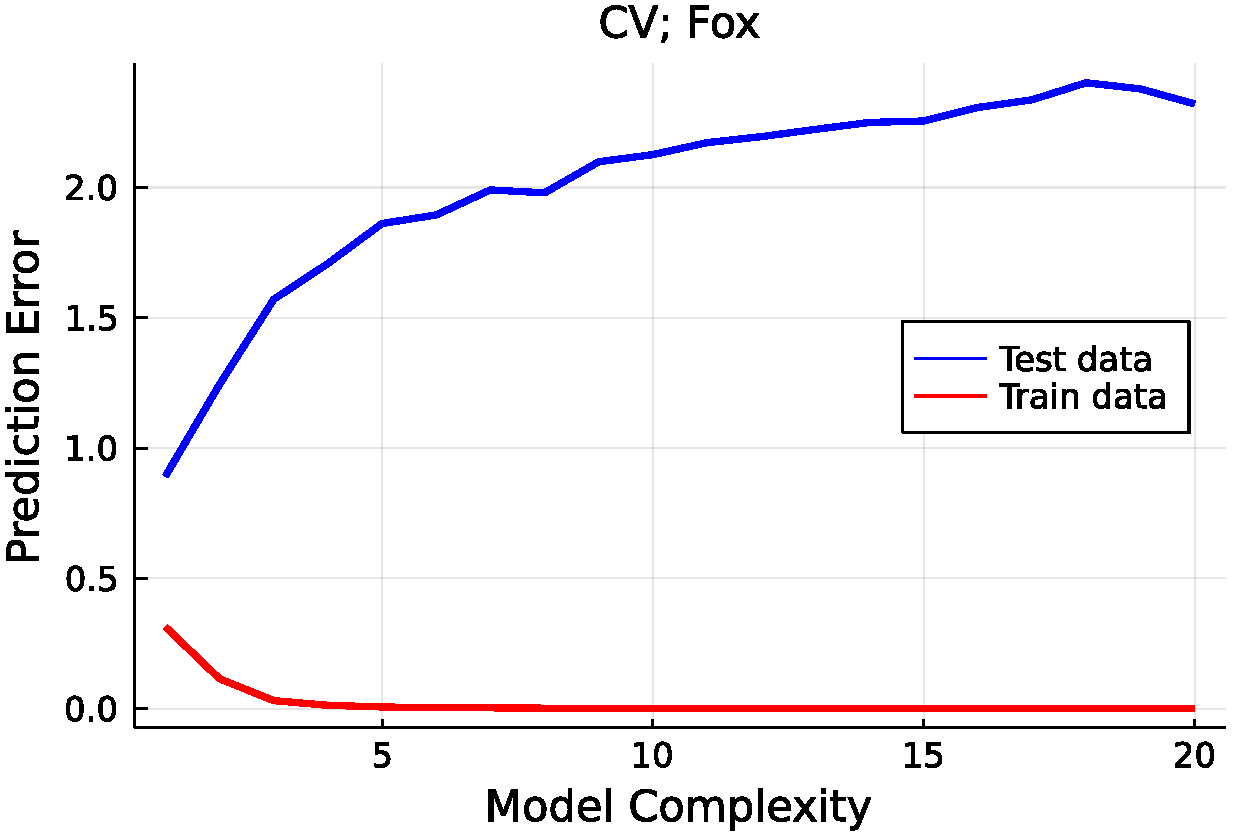
\includegraphics[width=8.0cm]{plots/Images/KFCV_Fox.pdf} }}%
	\subfloat[CV for dataset Tiger.]
	{{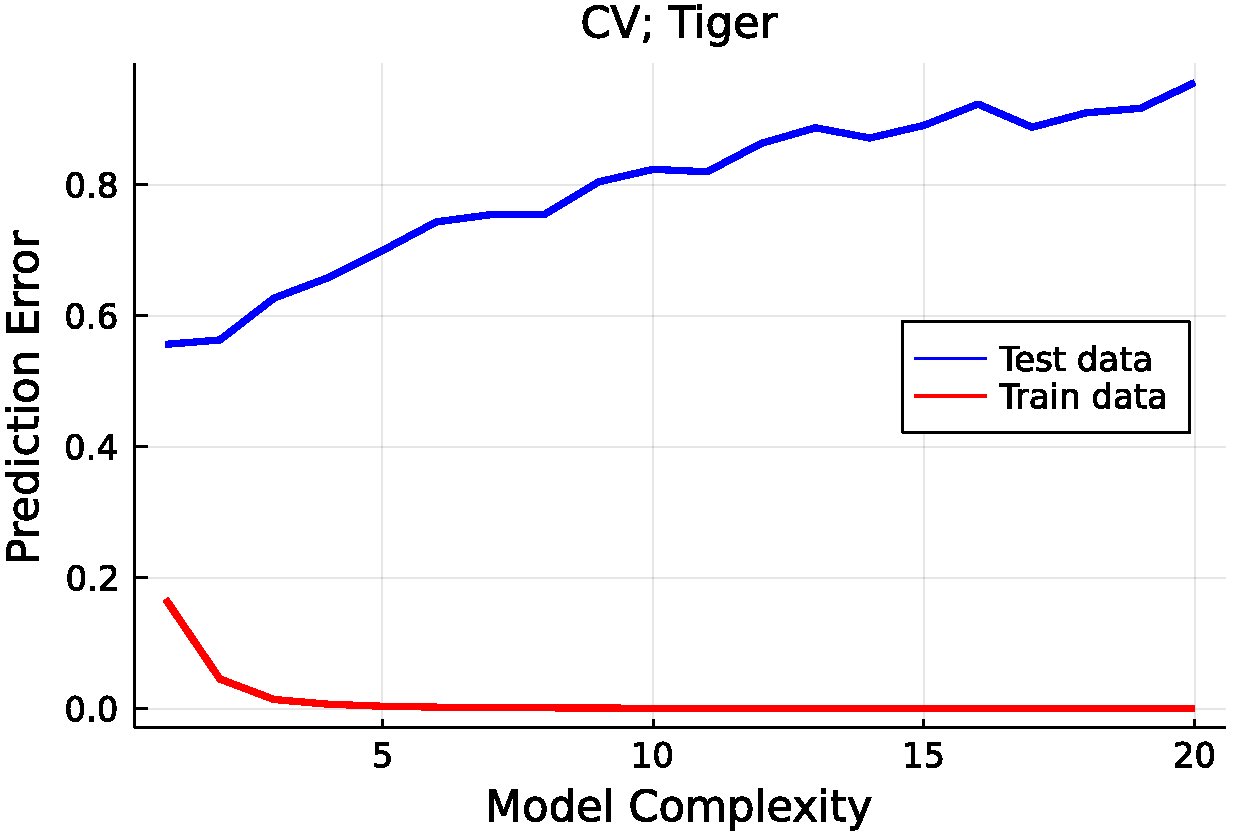
\includegraphics[width=8.0cm]{plots/Images/KFCV_Tiger.pdf} }}%
	\caption{Evaluation of prediction error with the use of training data and testing data on MIL datasets Musk1, Musk2, Fox and Tiger. }%
	\label{CV}%
\end{figure}

\begin{table}[h]
	\centering
	\begin{tabular}{|l|l|l|l|}
		\hline
		Dataset  &$\argmin \widehat{\mathrm{Err}}(z)$ & $ \min \widehat{\mathrm{Err}}(z)$ &$\widehat{\mathrm{Err}}(z=10)$ \\ \hline
		Musk1              & 2        & 0.70& 0.97   \\ \hline
		Musk2              & 3        & 0.57& 0.81   \\ \hline
		Fox               & 1        & 0.89 &  2.13 \\ \hline
		Tiger               & 1        & 0.56  & 0.82    \\ \hline
	\end{tabular}
	\caption{Results of CV evaluated on the testing data.}
	\label{tab:resultsCV}
\end{table}




\section{MIL to HDGM problem}
In the previous part was performed the CV experiment with expected results. However, the estimated prediction error seems to be rather high. Logically, the question has been raised whether the prediction error can be reduced and also whether it is possible to make $r$ smaller.
\subsection{Setup}
On the initiative of reducing the prediction error, it is proposed to train a MIL model that is obtained by minimizing the hybrid loss function 

\begin{equation}
	\min_{\boldsymbol{\theta}}- \mathbb{E}_{p_{\mathrm{data}}(\boldsymbol{x},y)}\left[\alpha\log \frac{\exp\left({f_{\boldsymbol{\theta}}\left(\boldsymbol{x}\right)[y]}\right)}{\sum_{i=1}^C\exp\left({f_{\boldsymbol{\theta}}\left(\boldsymbol{x}\right)[y_i]}\right)}+ \left(1-\alpha\right)\log \frac{\exp\left({f_{\boldsymbol{\theta}}\left(\boldsymbol{x}_i\right)[y]}\right)}{\sum_{j=1}^N\exp\left({f_{\boldsymbol{\theta}}\left(\boldsymbol{x}_j\right)[y]}\right)} \right].
	\end{equation}
Since the discriminative part is already used in HMill framework, the only task is to add the generative part into it. At this point are available all normalization samples, thus $M=N$. This modification should lead to a reduced prediction error evaluated on training data.\\
In the first part of this experiment, we would like to train models in relation to parameter $\alpha$. For this setup, we need to choose fixed $z$. Since authors of \cite{mandlik} usually use $z=10$, we use this value as well. For the prediction error evaluation is used standard cross--entropy as in the previous experiment, again with $r=100$ and $\alpha \in \left\{0.0, 0.1, 0.2,\dots,1.0\right\}$. Therefore estimated prediction error can be written in the form
\begin{equation}
	\widehat{\mathrm{Err}}(\alpha) = \frac{1}{r}\sum_{k=1}^r \pazocal{L}_k(z=10, \alpha).
\end{equation}
We hope to see a curve in the shape of a bowl, having its global minimum in a point $\alpha=0.5$ or somewhere near.\\ 
In the second part, evaluating of the prediction error is approached the other way. Fixed $\alpha = 0.5$ is selected and the dependency on $z~\in~\left\{1,2,3\dots,20 \right\}$ is evaluated as in the section \ref{experimentCV}. Finally, estimated prediction error in this case is defined by
\begin{equation}
	\widehat{\mathrm{Err}}(z) = \frac{1}{r}\sum_{k=1}^r \pazocal{L}_k(z, \alpha =0.5).
\end{equation}
In other words, the setup is the same as in the \ref{experimentCV}, therefore obtained results will be added to the Figure \ref{CV} and table \ref{tab:resultsCV} for a convenient comparison. Note that curves for train data from this experiment will be omitted, since they are not important at this point. We are only interested in predictions for test data.  
\clearpage
\subsection{Results}



Results of the first part are represented in Figure \ref{fig:HDGE} and in Table \ref{tab:resultsHDGE}, where can be seen that adding the generative term into the MIL loss function decreased the prediction error evaluated on all datasets. This improvement is considerable on datasets Musk1 and Musk2, where a can be seen a nice bowl. On datasets Fox and Tiger such improvement does not occur. This means that HDGM approach works, thus a regularization in the form of very simple generative term may bring improvement in predictions. Unfortunately, the choice of $\alpha=0.5$ was not confirmed as the best in our experiment, see Table \ref{tab:resultsHDGE}.   \\
In the second part of the experiment results are shown in Figure \ref{fig:resultsHDGMz} and in Table \ref{tab:HDGMz}. Here is the situation very similar to the previous part of this experiment. Improvement of the prediction error is quite noticeable on first two datasets Musk1 and Musk2, while Fox and Tiger does not look so convincingly. In addition, number of random splits $r=100$ is still needed to get rid of the noise on the prediction error. \\
Overall, it can be said that HDGM approach leads to the decreased prediction error in a small way. 
\begin{table}[h]
	\centering
	\begin{tabular}{|l|l|l|l|}
		\hline
		Dataset  &  $\argmin \widehat{\mathrm{Err}}(\alpha)$& $\min \widehat{\mathrm{Err}}(\alpha)$ \\ \hline
		Musk1              & 0.4      & 0.68   \\ \hline
		Musk2             & 0.2      & 0.54   \\ \hline
		Fox                 & 0.7      & 1.89  \\ \hline
		Tiger            & 0.4      & 0.74      \\ \hline
	\end{tabular}
	\caption{Prediction error statistics for HDGM in case of $z=10$.}
	\label{tab:resultsHDGE}
\end{table}
\begin{figure}[h]
	\centering
	\subfloat[HDGM for dataset Musk1.]
	{{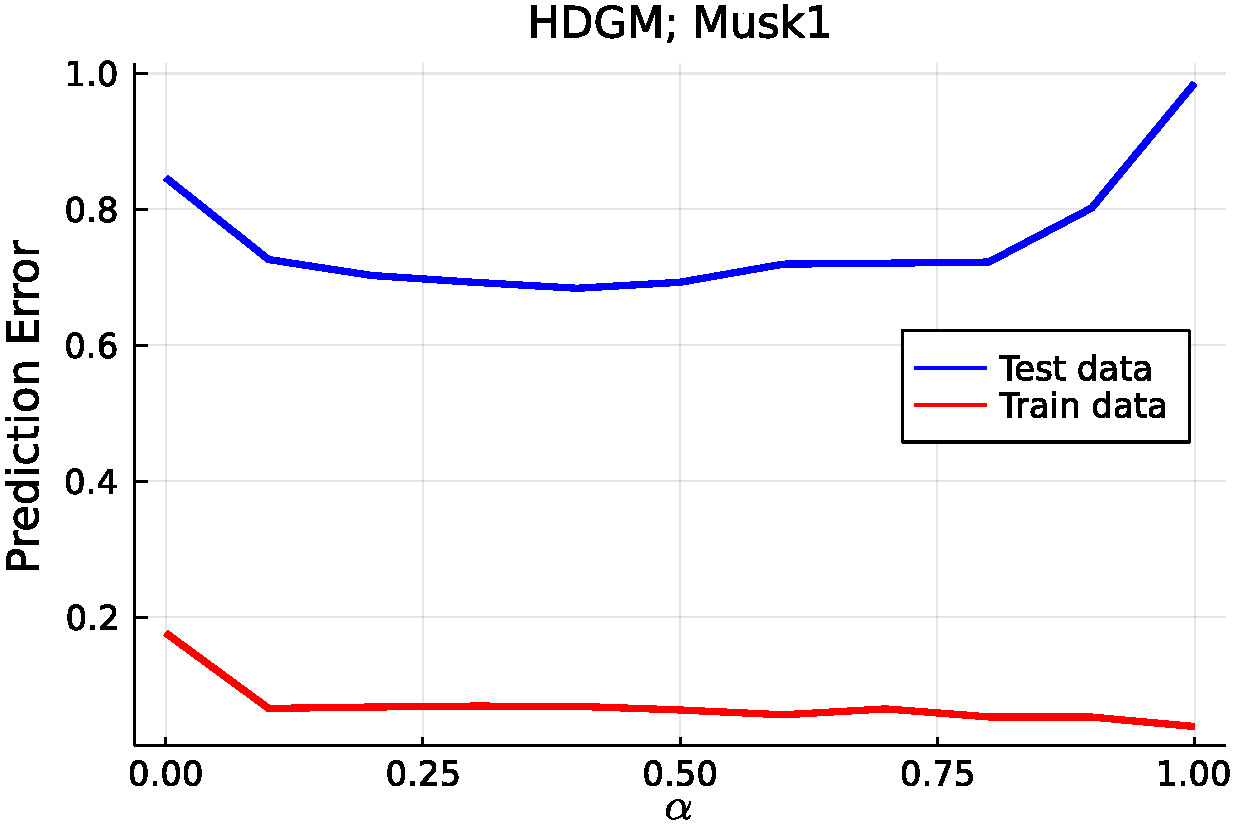
\includegraphics[width=8.2cm]{plots/Images/HDGM_Musk3.pdf} }}%
	\subfloat[HDGM for dataset Musk2.]
	{{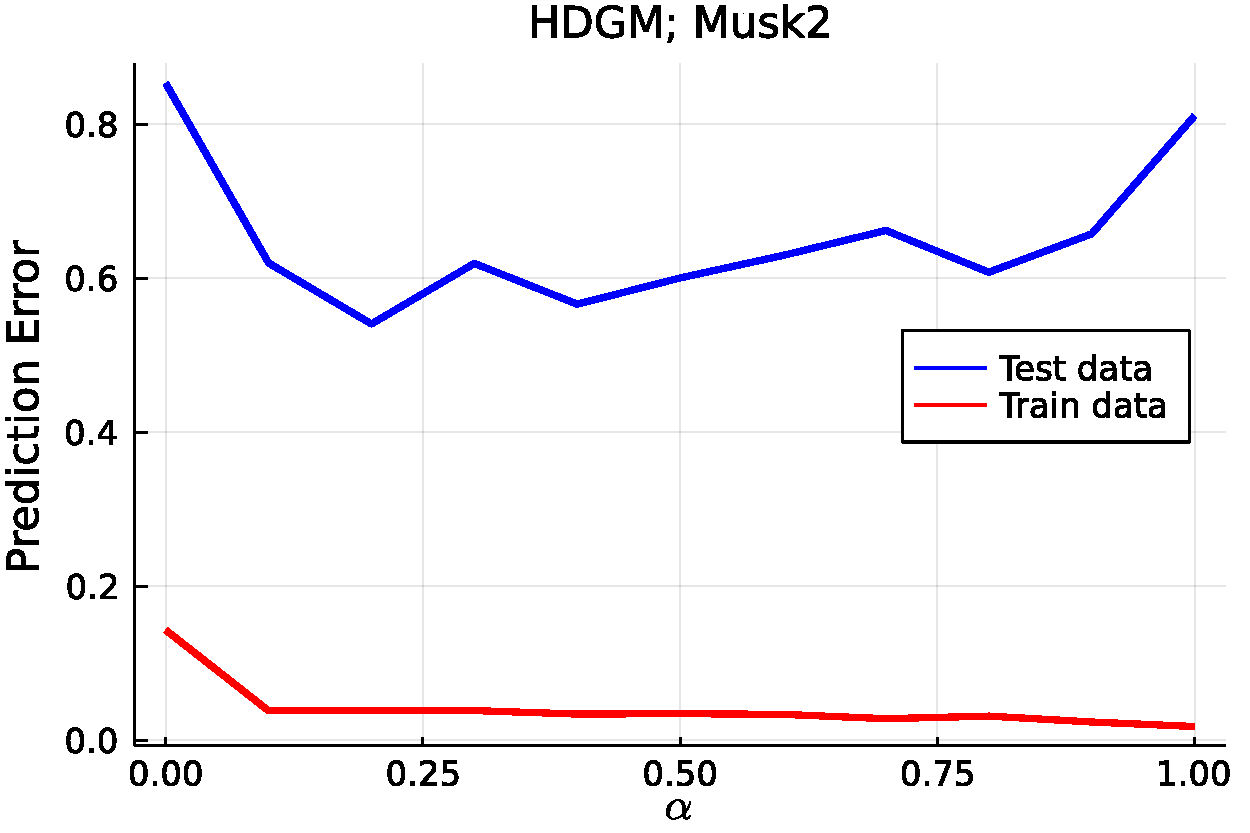
\includegraphics[width=8.2cm]{plots/Images/HDGM_Musk4.pdf} }}%
	\
	\subfloat[HDGM for dataset Fox.]
	{{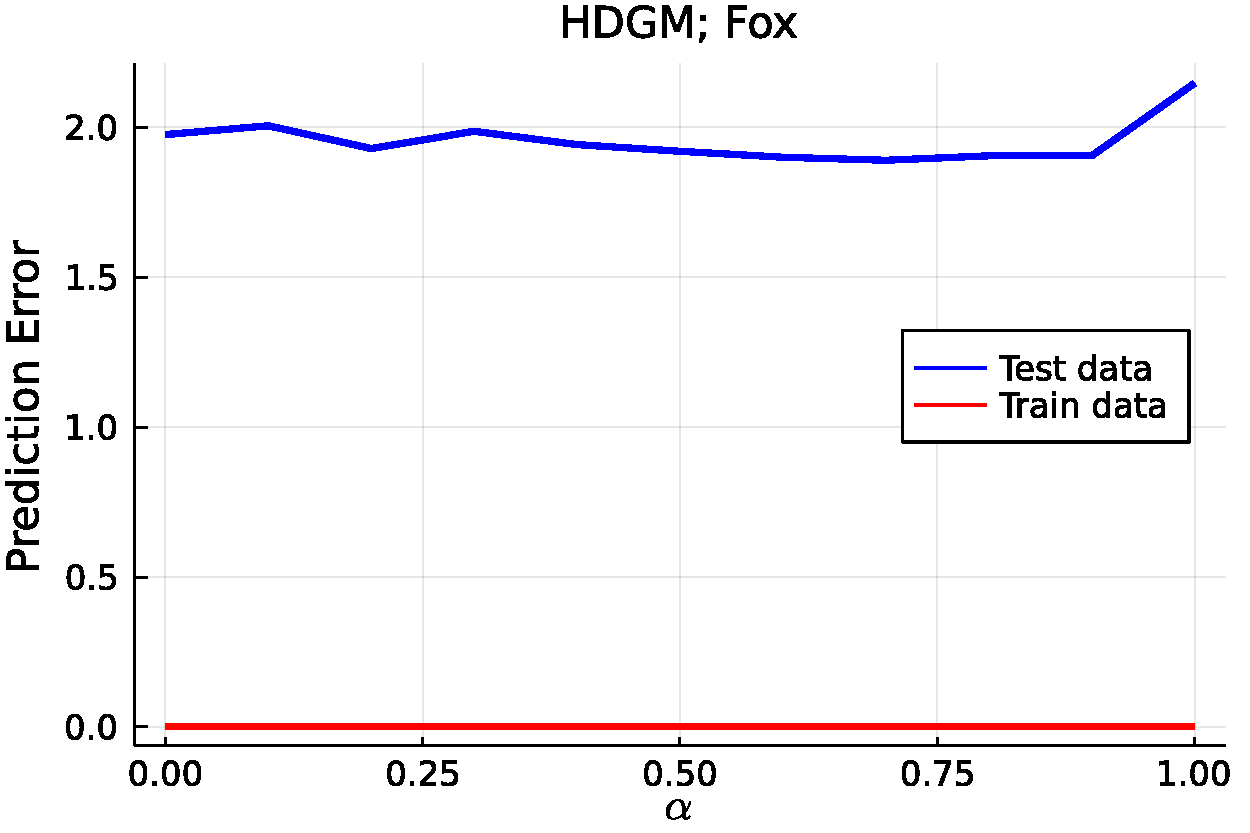
\includegraphics[width=8.2cm]{plots/Images/HDGM_Fox.pdf} }}%
	\subfloat[HDGM for dataset Tiger.]
	{{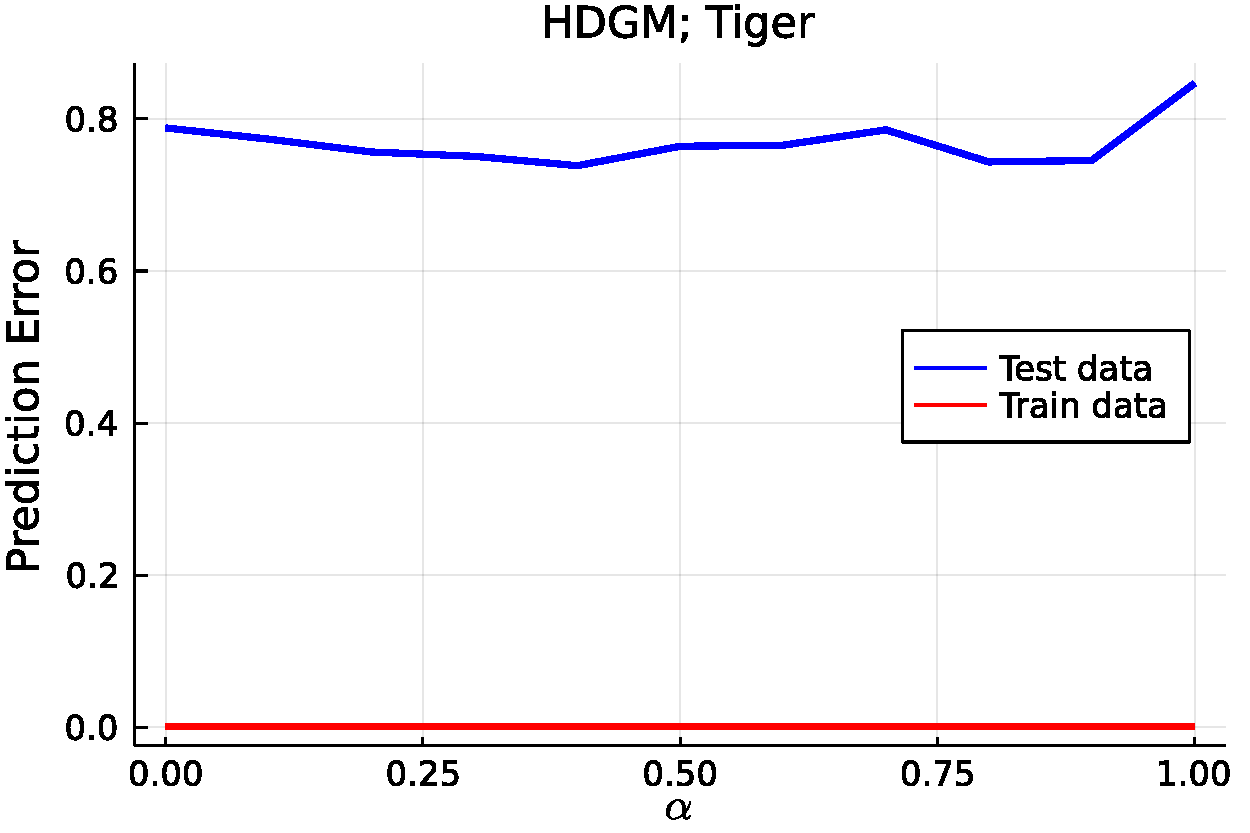
\includegraphics[width=8.2cm]{plots/Images/HDGM_Tiger.pdf} }}
	\caption{Evaluation of the prediction error $\widehat{\mathrm{Err}}(\alpha)$ with the use of training data and testing data on MIL datasets. }%
	\label{fig:HDGE}%
\end{figure}


\begin{table}[h]
	\centering
	\begin{tabular}{|l|l|l|l||l|l|l|}
		\hline
		& \multicolumn{3}{l||}{~~~~~~~~~~~\textbf{Discriminative part only}} & \multicolumn{3}{l|}{~~~~~~~~~~~~~~~~~\textbf{HDGM}; $\alpha=0.5$} \\ \hline
		Dataset & $\argmin \widehat{\mathrm{Err}}(z)$   & $\min \widehat{\mathrm{Err}}(z)$ &$\widehat{\mathrm{Err}}(z=10)$  &   $\argmin \widehat{\mathrm{Err}}(z)$             &     $\min \widehat{\mathrm{Err}}(z)$       &     $\widehat{\mathrm{Err}}(z=10)$         \\ \hline
		Musk1   & 2             & 0.70         & 0.97    &    6          &  0.64           &  \textbf{0.69}           \\ \hline
		Musk2   & 3              & 0.57         & 0.81    &    6          & 0.55            &  \textbf{0.66}           \\ \hline
		Fox     & 1              & 0.89         & 2.13    &    1          &  0.95           &   \textbf{1.96}          \\ \hline
		Tiger   & 1              & 0.56          & 0.82       &   2           &   0.58          &   \textbf{0.80}          \\ \hline
	\end{tabular}
	\caption{Comparison of prediction error statistics for HDGM $\alpha=0.5$ and discriminative part only. Pay attention especially to the last column in each approach, $\widehat{\mathrm{Err}}(z=10)$.}
	\label{tab:HDGMz}
\end{table}

\begin{figure}[h]
	\centering
	\subfloat[HDGM: $\alpha=0.5$ vs Discriminative; Musk1.]
	{{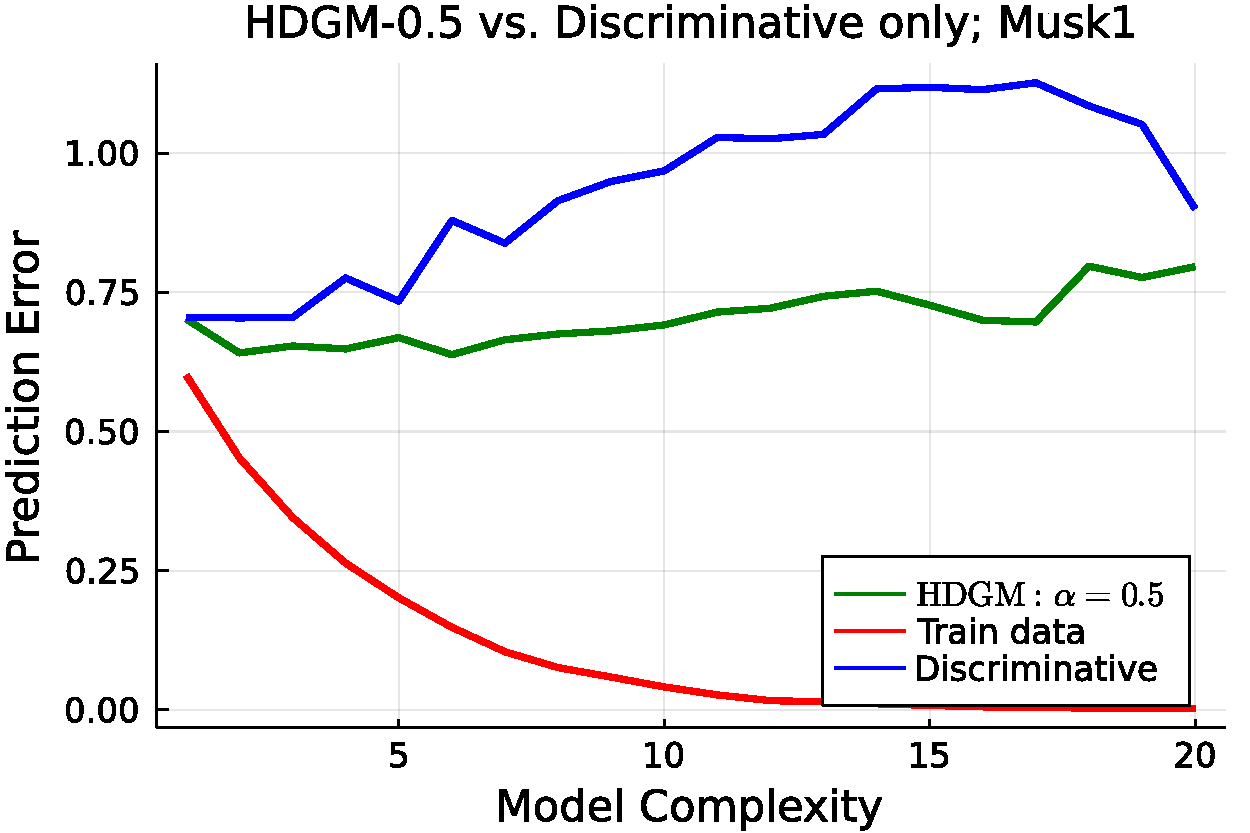
\includegraphics[width=8.2cm]{plots/Images/supervisedvsHDGM0_5_Musk1.pdf} }}%
	\subfloat[HDGM: $\alpha=0.5$ vs Discriminative; Musk2.]
	{{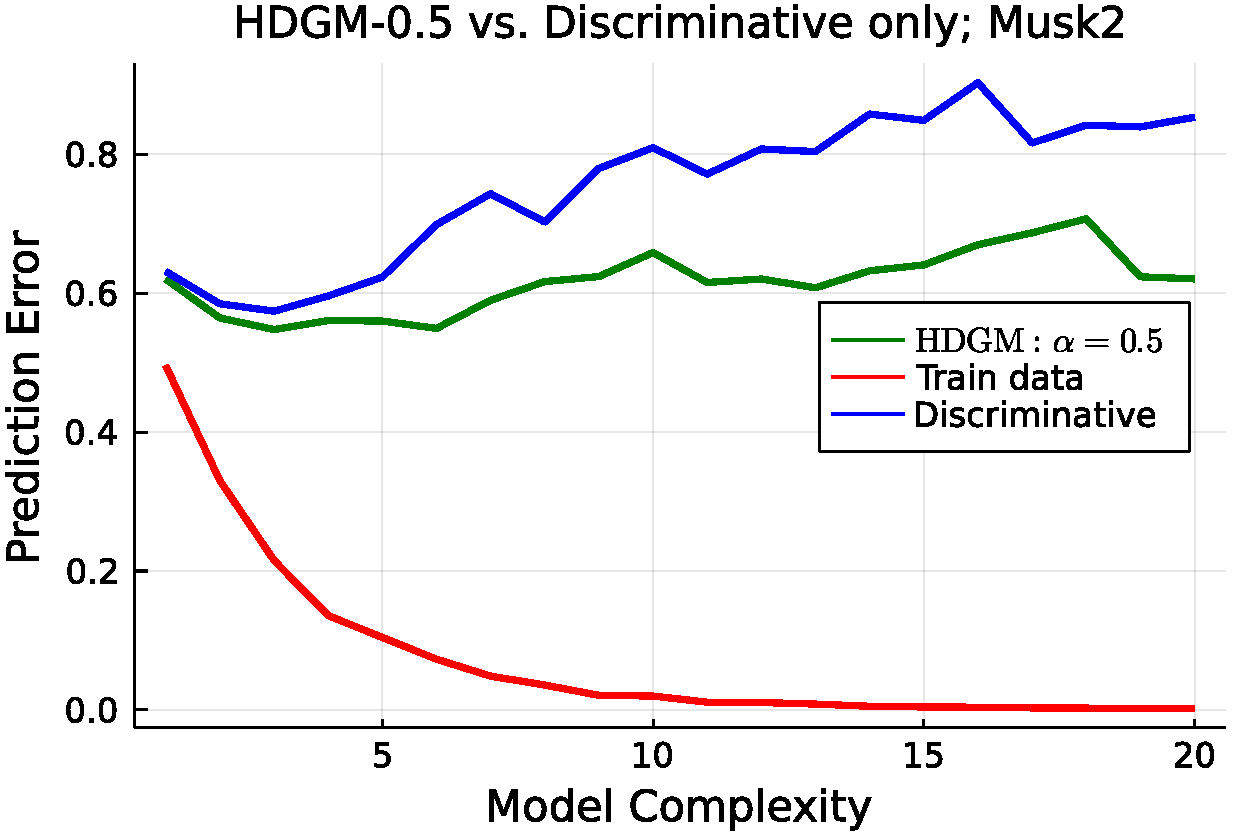
\includegraphics[width=8.2cm]{plots/Images/supervisedvsHDGM0_5_Musk2.pdf} }}%
	\
	\subfloat[HDGM: $\alpha=0.5$ vs Discriminative; Fox.]
	{{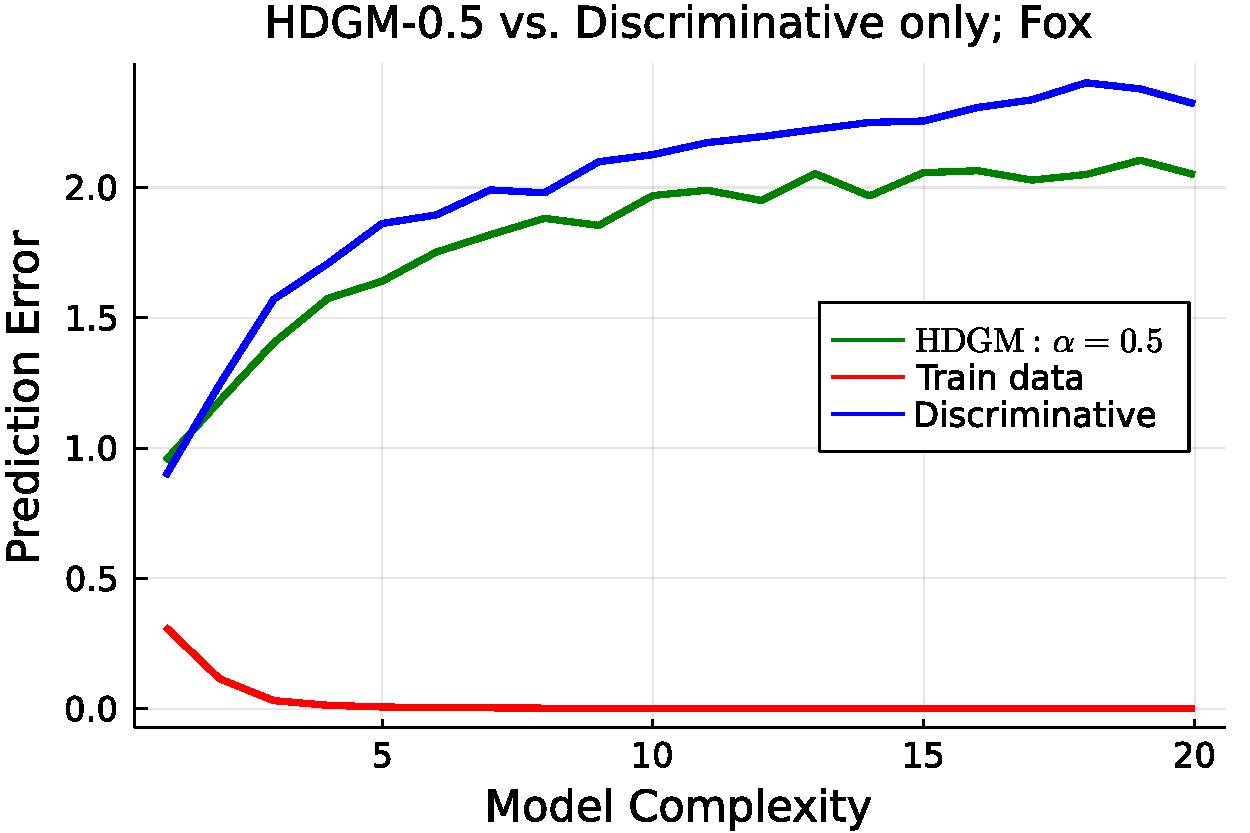
\includegraphics[width=8.2cm]{plots/Images/supervisedvsHDGM0_5_Fox.pdf} }}%
	\subfloat[HDGM: $\alpha=0.5$ vs Discriminative; Tiger.]
	{{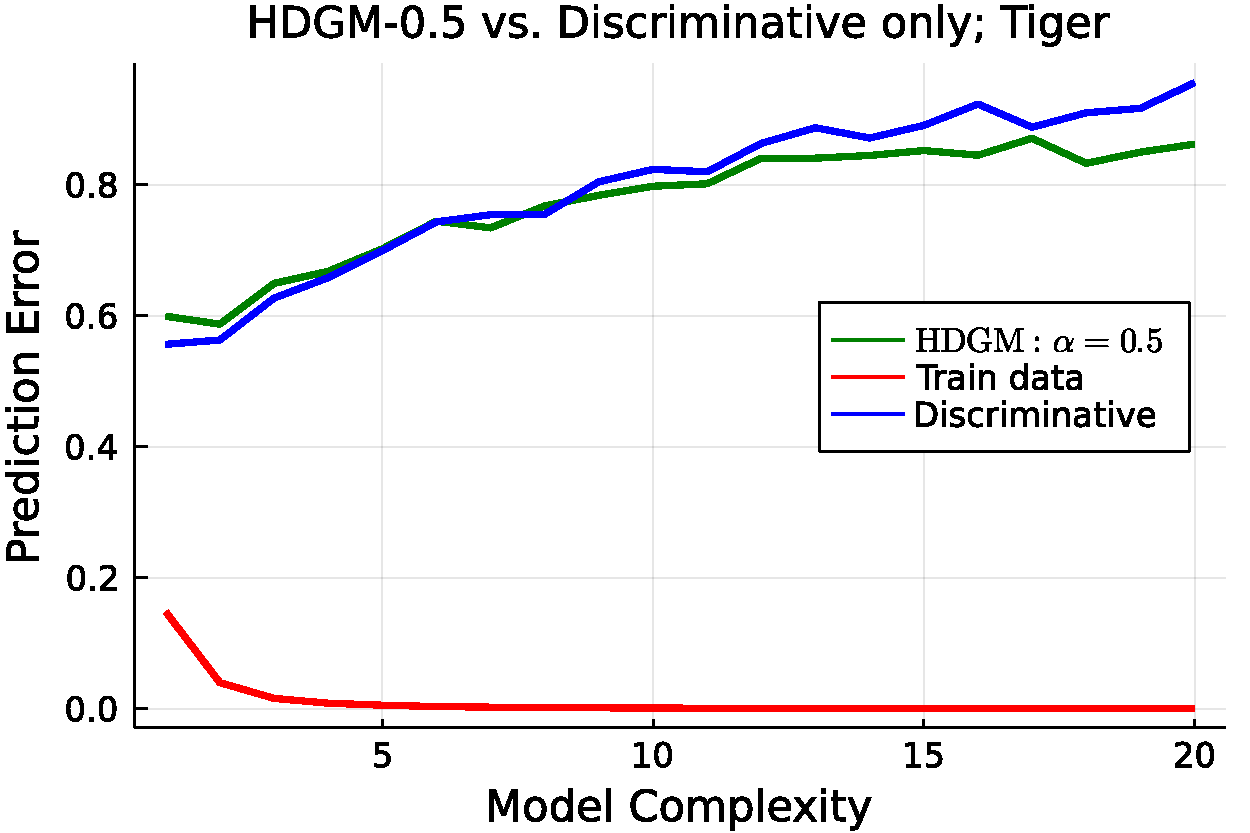
\includegraphics[width=8.2cm]{plots/Images/supervisedvsHDGM0_5_Tiger.pdf} }}
\caption{Comaparison of the prediction error  $\widehat{\mathrm{Err}}(z)$ for HDGM $\alpha=0.5$ and discriminative part only. }%
	\label{fig:resultsHDGMz}%
\end{figure}
